\newpage
\chapter{Пакетна организация и основни операции в R}
\label{chapter02}

Най-голямата сила на продукта R се дължи на хилядите пакети (софтуерни приставки), създадени от безброй потребители на продукта. Наличните пакети покриват цялата област на статистиката и статистическата обработка на данни. 

Под пакет се разбира софтуерна библиотека от предварително написан програмен кой, който има за цел да реши определена задача или група от задачи. Тъй като продуктът R е една отворена система е важно да се има предвид, че не всички пакети са с еднакво качество. Една част от пакетите са изключително професионално написани, устойчиви са на некоректно използване и имат добра база от поддържащи ги потребители. В същото време друга част от пакетите са създадени с голяма доза добри намерения, но работят бавно, дават дефекти или просто не вършат това за което са създадени. Голяма част от пакетите са написани от статистици за статистици и това може да доведе до някои странни въпроси при част от потребителите, особено при хора идващи от индустрията за производство на софтуер. 

Настоящото учебно помагало представя само най-основните пакети, достатъчни да бъде изложен материалът свързан с базовите познания по R. Опит да бъдат представени всички пакети е непосилен за едно издание, най-вече защото броят и видът на пакетите постоянно се променя. 

\section{Инсталиране на пакети}

Съществуват различни начини за инсталиране на пакети в R, но най-основният от тях е чрез команда в конзолата на пакета R. 

\begin{figure}[h!]
  \centering
  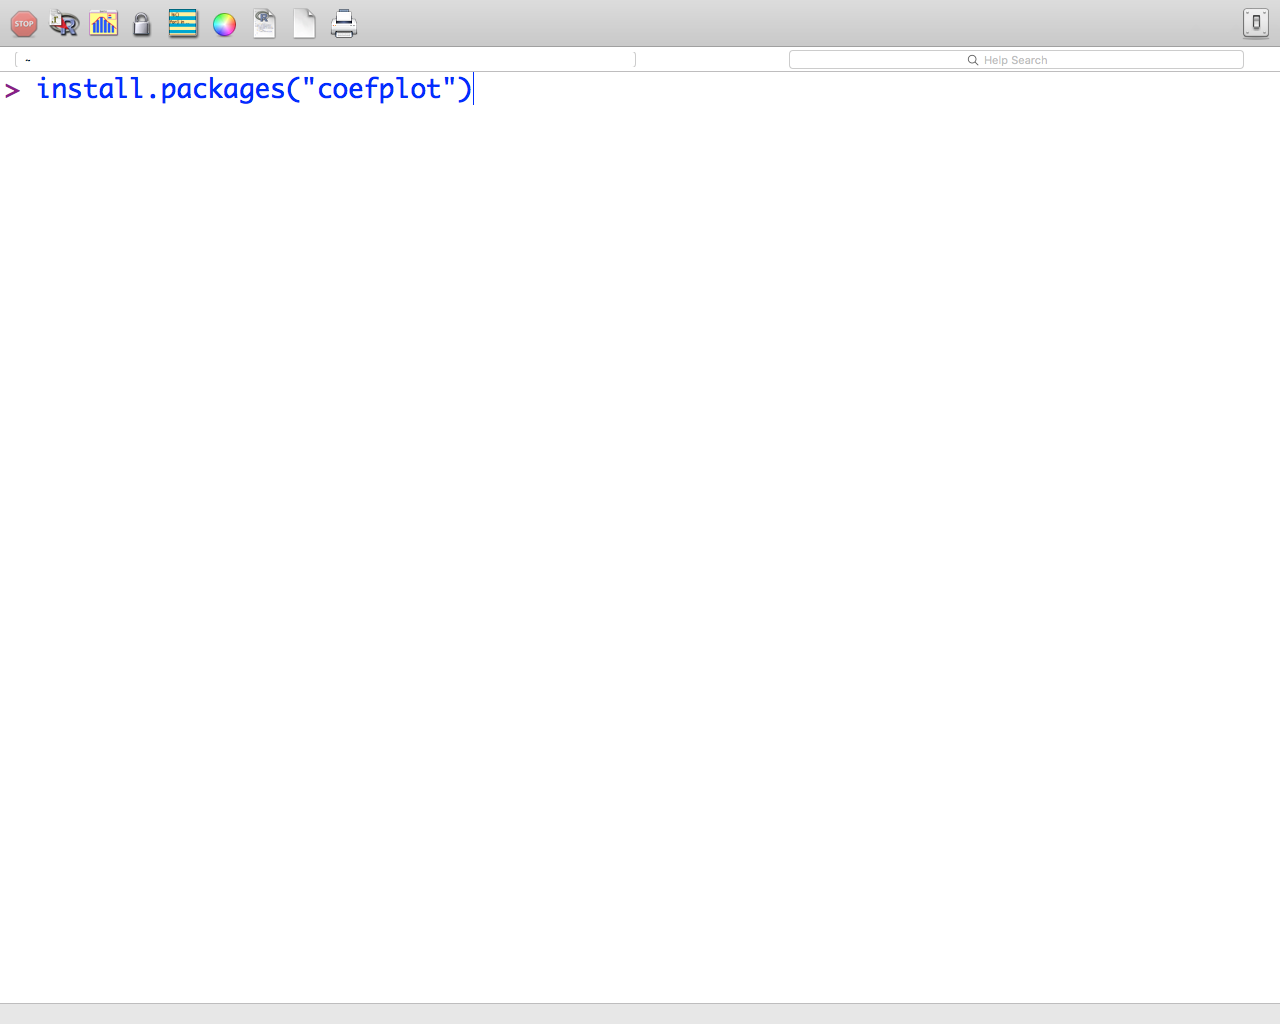
\includegraphics[width=1.0\linewidth]{pic0014}
  \caption{Команда за инсталиране на пакета coefplot}
\label{fig:pic0014}
\end{figure}
\FloatBarrier

За да започне инсталирането на пакет (в случая coefplot) е достатъчно да се изпише командата от Фиг. \ref{fig:pic0014}.

\begin{figure}[h!]
  \centering
  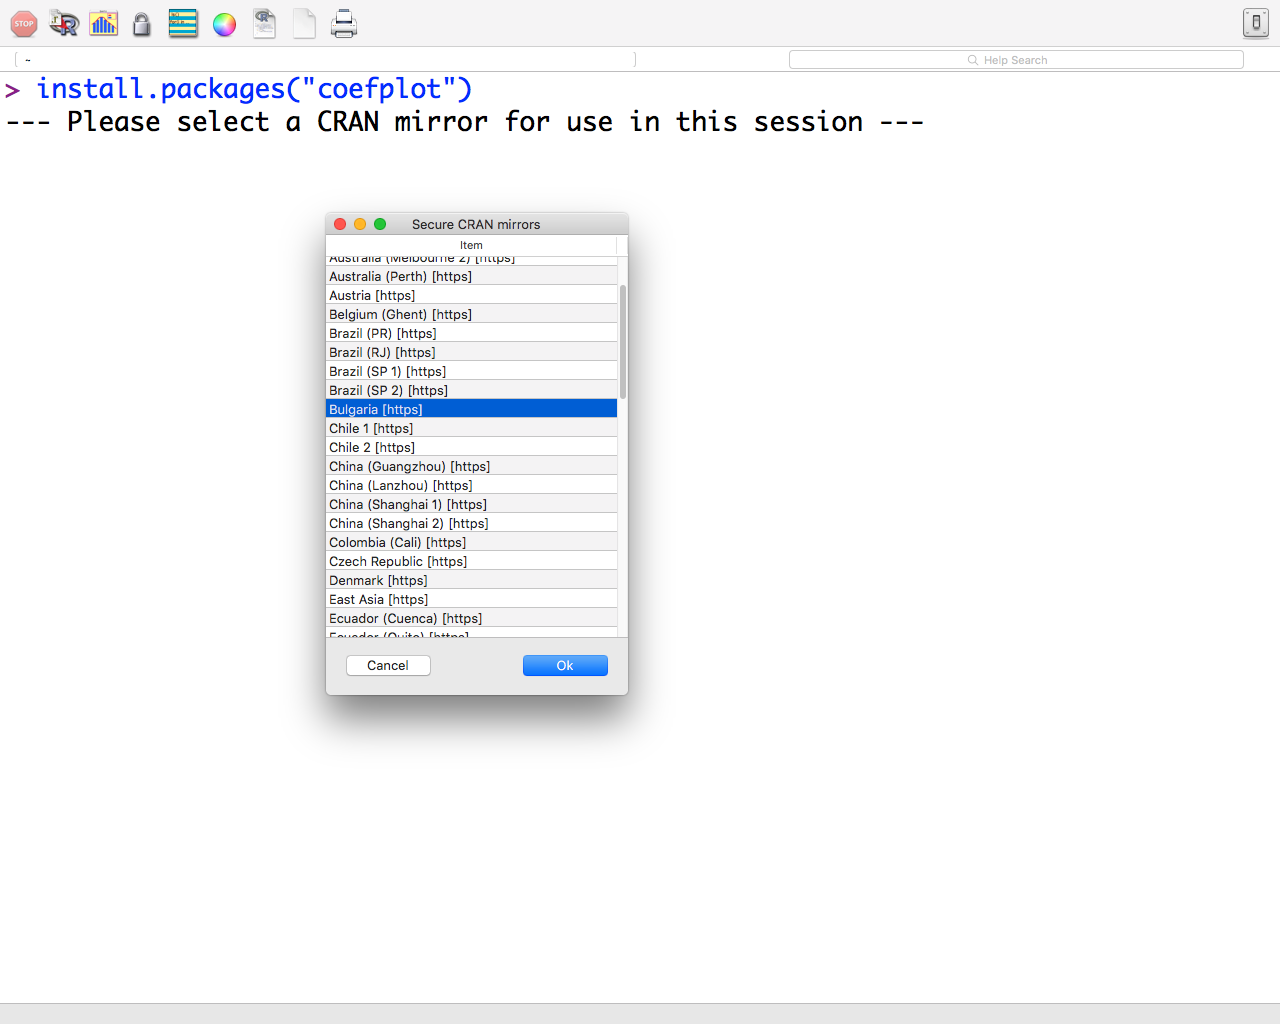
\includegraphics[width=1.0\linewidth]{pic0015}
  \caption{Избор на сървър за изтегляне на пакета}
\label{fig:pic0015}
\end{figure}
\FloatBarrier

След което следва избор на сървър за изтегляне на пакета (Фиг. \ref{fig:pic0015}). Разумна стратегия е да се избират сървъри, които териториално се намират в близост до мястото от което се работи. Това би осигурило малко по-голяма бързина на връзката в Глобалната мрежа. 

\begin{figure}[h!]
  \centering
  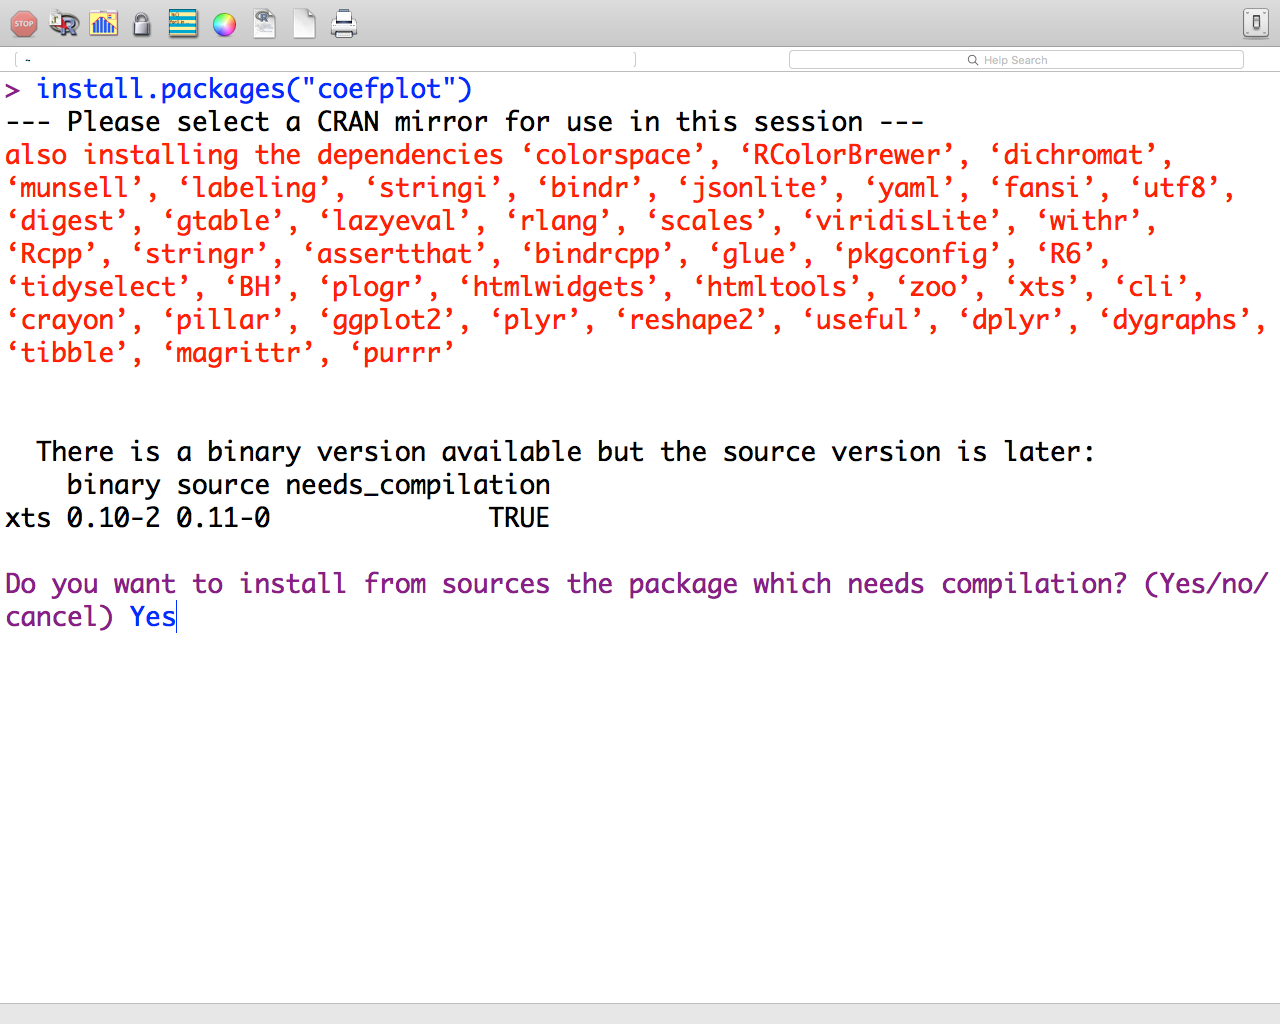
\includegraphics[width=1.0\linewidth]{pic0016}
  \caption{Зависимости между пакетите}
\label{fig:pic0016}
\end{figure}
\FloatBarrier

Често срещан случай е един пакет да има функционална зависимост от други пакети (Фиг. \ref{fig:pic0016}). В такава ситуация е необходимо всички нужни пакети също да бъдат инсталирани. Стратегията при разработка на пакети е те да бъдат предлагани в компилиран (бинарен) вид, но понякога най-новите версии са под формата на програмен код и тогава потребителят има възможност да избере между бинарната версия или версията с програмен код. 

\begin{figure}[h!]
  \centering
  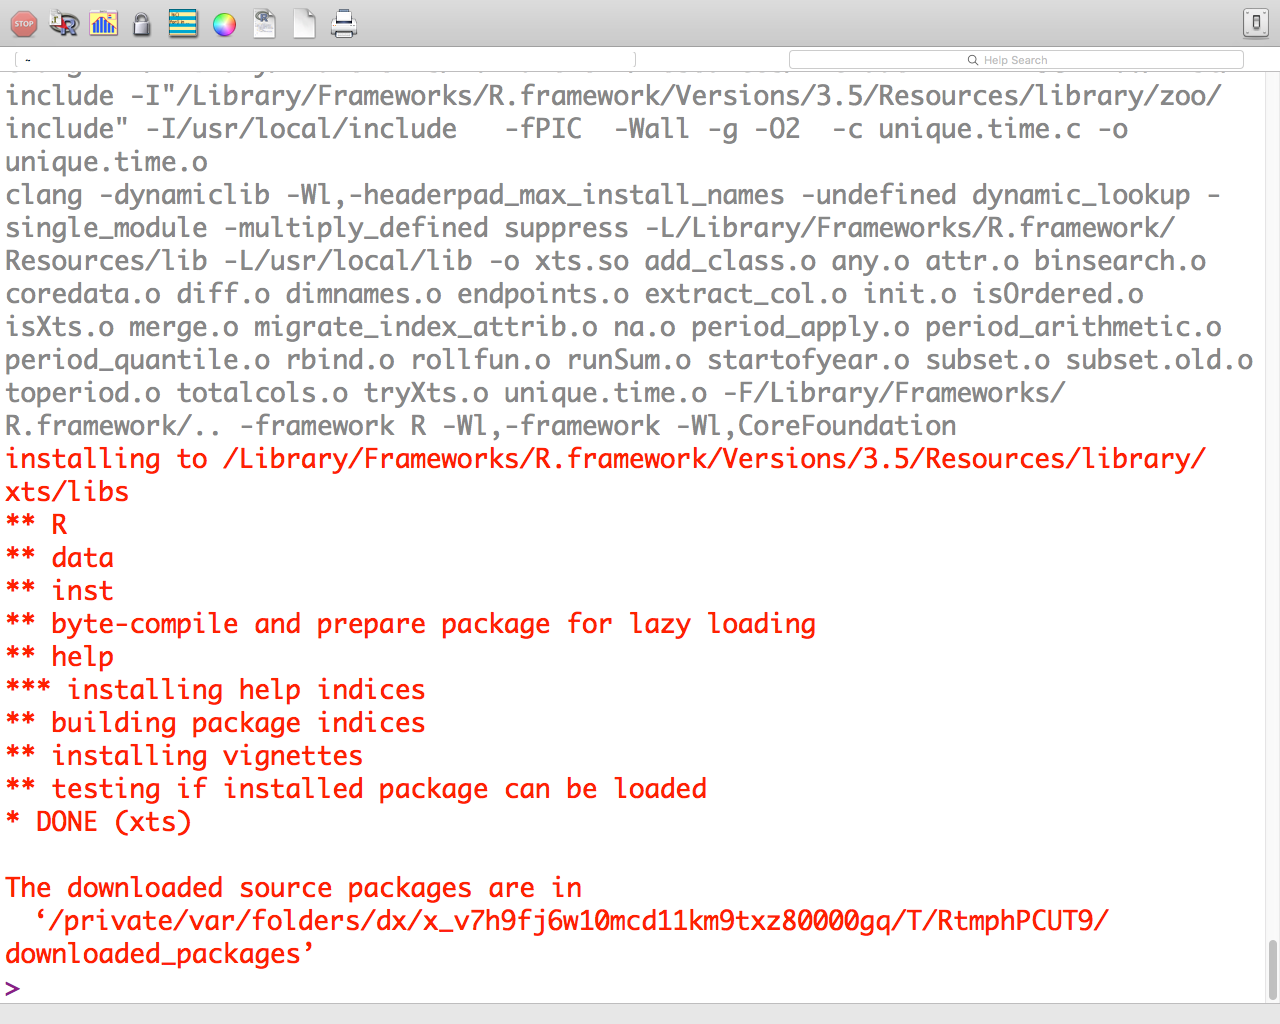
\includegraphics[width=1.0\linewidth]{pic0017}
  \caption{Резултат от инсталацията на пекета}
\label{fig:pic0017}
\end{figure}
\FloatBarrier

Инсталацията на пакета приключва с подробен листинг, съдържащ описание на извършените операции (Фиг. \ref{fig:pic0017}). 

\begin{figure}[h!]
  \centering
  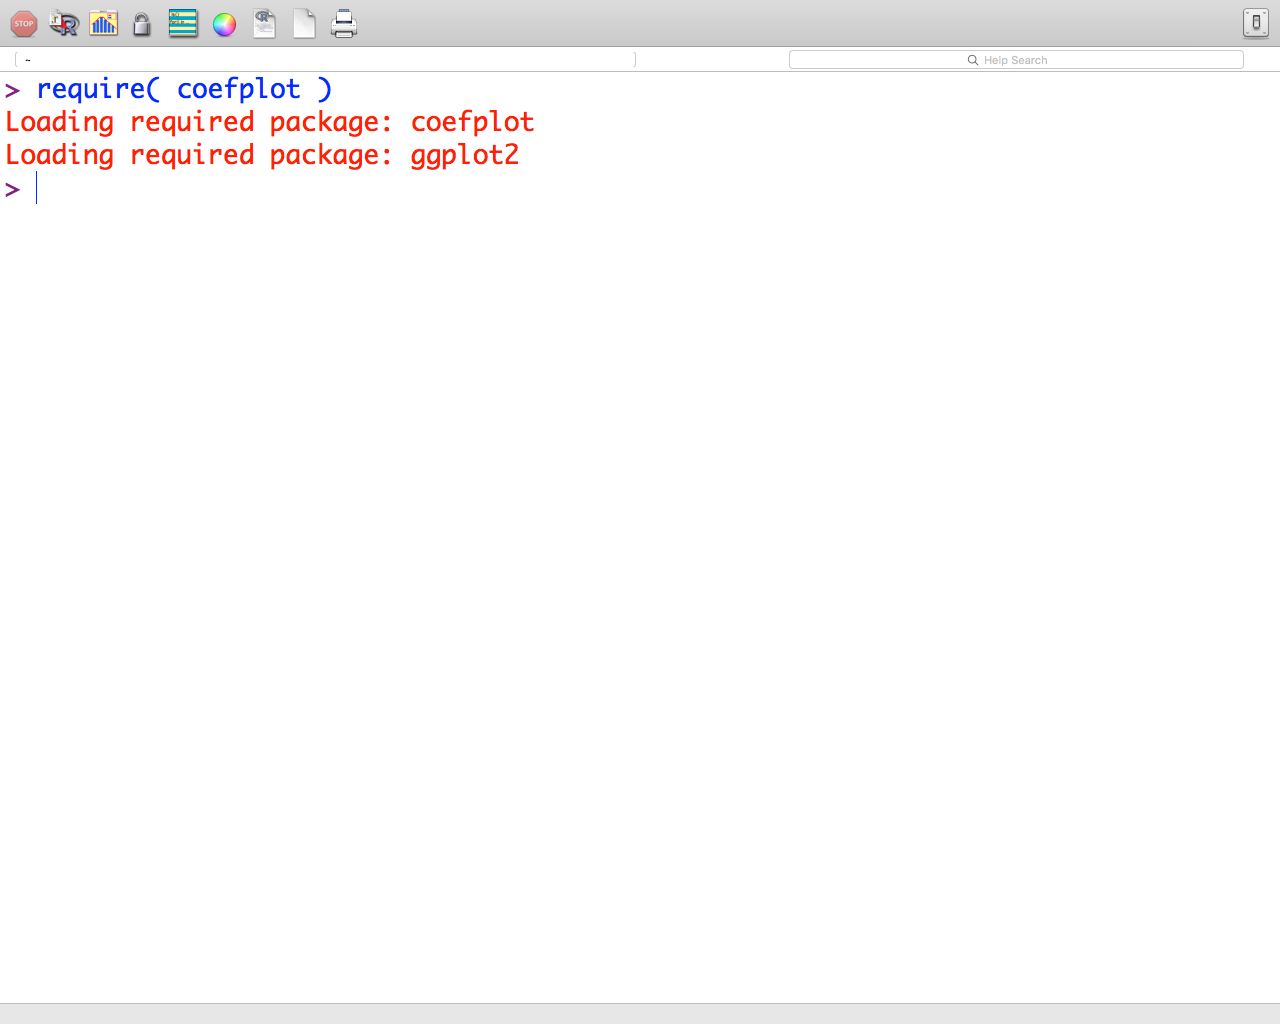
\includegraphics[width=1.0\linewidth]{pic0018}
  \caption{Зареждане на пакета coefplot}
\label{fig:pic0018}
\end{figure}
\FloatBarrier

Дали пакетът е надлежно инсталиран може да се провери с командата require (Фиг. \ref{fig:pic0018}), която зарежда пакета в паметта. 

Съществува възможност пакетите да се инсталират под формата на програмен код, директно от хранилищата за програмен код, но за тази цел са нужни подходящите компилатори (най-често C/C++ и Fortran), както и по-задълбочени умения по програмиране. В редки случаи се налага инсталиране на пакета от ZIP файл. При такава ситуация е важно предварително да бъдат инсталирани всички пакети от които инсталирания пакет зависи. 

Премахване на инсталирани пакети става с помощта на командата remove.packages на която се подава вектор с имената на пакетите, които трябва да бъдат премахнати.

\section{Зареждане на пакети}

За да бъдат използвани пакетите не е достатъчно те да бъдат инсталирани, но трябва с команда да бъдат включени в текущата сесия от изчисления. R предлага две команди за зареждане на пакети – library и require. И двете изпълняват едно и също нещо – зареждат пакета в общата памет. Разликата е, че require връща TRUE, ако зареждането е било успешно и FALSE при неуспех. Тази възможност е полезна в редките случаи, когато пакетът се зарежда от програмния текст на функция. Подобна практика не е препоръчителна, но R дава такава възможност. И двете функции получават като параметър името на пакета, със или без кавички. Пакетите се зареждат еднократно и остават налични през цялата сесия от изчисления или докато изрично не бъдат премахнати от общата памет. 

\begin{figure}[h!]
  \centering
  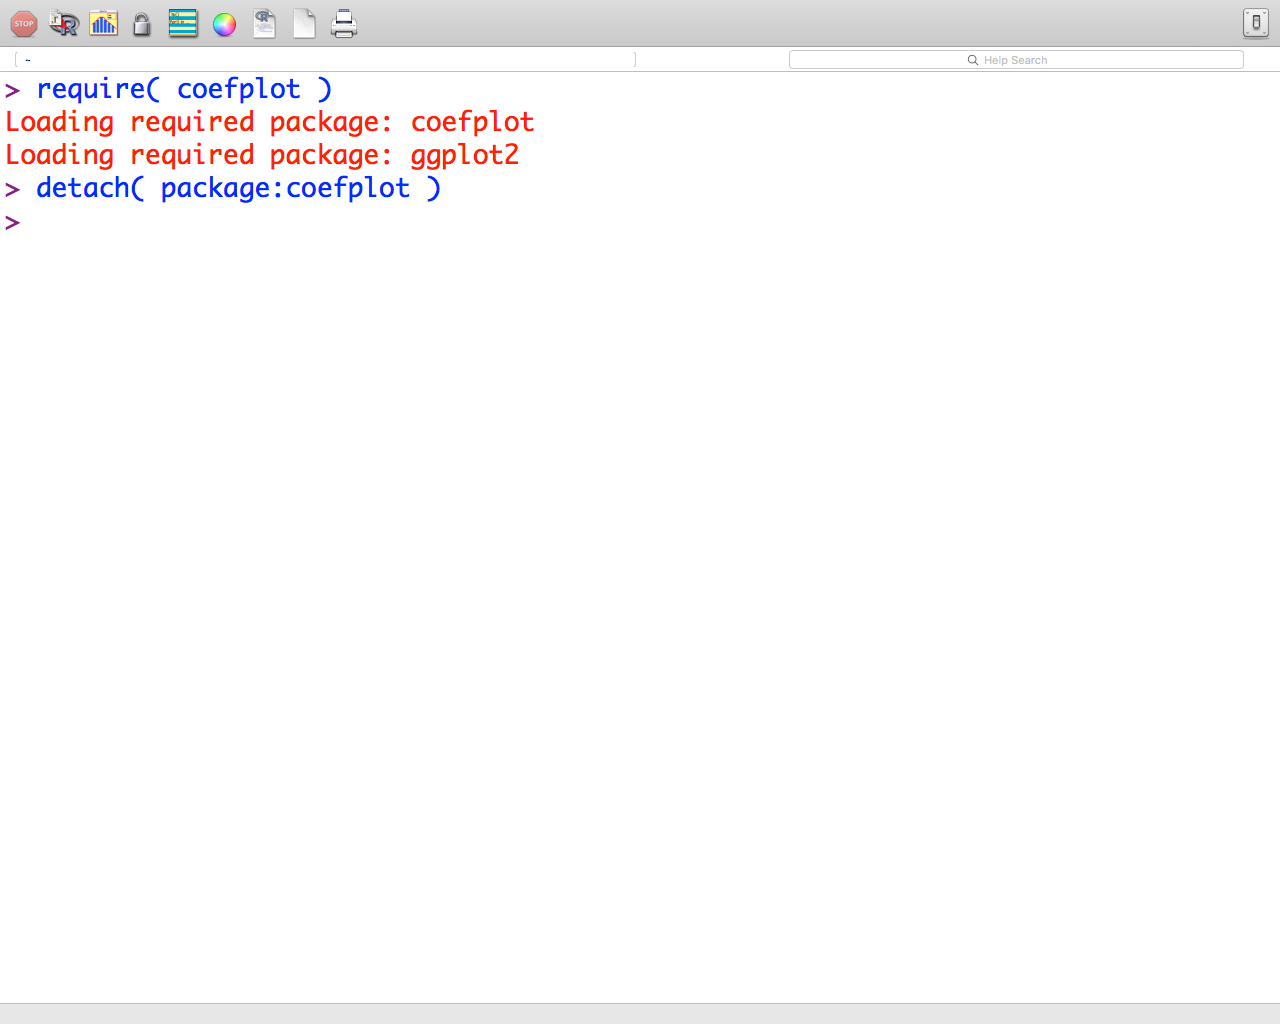
\includegraphics[width=1.0\linewidth]{pic0019}
  \caption{Премахване на пакета coefplot от общата памет}
\label{fig:pic0019}
\end{figure}
\FloatBarrier

Премахването на пакет от общата памет става с командата detach (Фиг. \ref{fig:pic0019}). Същественото при тази команда е, че преди името на пакета се записва думата package. 

Тъй като пакетите се разработват основно на доброволни начала не рядко се случва в различни пакети да има едноименни функции. При подобна колизия на имената решението е операцията за принадлежност – двойно двуеточие (::). Когато бъде използвана операцията за принадлежност дори може да не се зарежда пакетът към който принадлежи функцията. 

\section{Основни математически операции}

